\documentclass[10pt]{article}

\usepackage[margin=0.75in]{geometry}
\usepackage{amsmath,amsthm,amssymb,bm}
\usepackage{xcolor}
\usepackage{cancel}
\usepackage{graphicx}
\usepackage{changepage}
\usepackage{circuitikz}
\usepackage{pgfplots}
\usepackage{minted}
\usepackage{physics}
\usepackage{hyperref}
\usepackage{subcaption}
\usepackage{tikz}
\usepackage{tikz-3dplot}
\usepackage{siunitx}
\usepackage{fontspec}
\usepackage{relsize}
\usepackage{todonotes}
\usepackage{multicol, multirow, booktabs}
\usepackage[breakable]{tcolorbox}
\usepackage[inline]{enumitem}

\theoremstyle{definition}
\newtheorem{problem}{Problem}
\newtheorem{soln}{Solution}

\pgfplotsset{compat=newest}
\usetikzlibrary{lindenmayersystems}
\usetikzlibrary{arrows}
\usetikzlibrary{calc}
\usetikzlibrary{positioning, fit}
\usetikzlibrary{3d, perspective}
\usetikzlibrary{math}
\usetikzlibrary{fadings}
\usetikzlibrary{angles,quotes} 

\definecolor{incolor}{HTML}{303F9F}
\definecolor{outcolor}{HTML}{D84315}
\definecolor{cellborder}{HTML}{CFCFCF}
\definecolor{cellbackground}{HTML}{F7F7F7}
\newcommand{\ui}{\hat{i}}
\newcommand{\uj}{\hat{j}}
\newcommand{\uk}{\hat{k}}
\newcommand{\ux}{\hat{\mathbf{x}}}
\newcommand{\uy}{\hat{\mathbf{y}}}
\newcommand{\uz}{\hat{\mathbf{z}}}
\newcommand{\uv}[1]{\hat{\bv{{#1}}}}
\newcommand{\pr}[1]{{#1^\prime}}
\newcommand{\pd}[2][]{{\frac{\partial^{#1}}{\partial {{#2}^{#1}}}}}
\newcommand{\dif}[2][]{{\frac{d^{#1}}{d{{#2}^{#1}}}}}
\pgfdeclarelayer{background}  
\pgfsetlayers{background,main}
\AtBeginDocument{\RenewCommandCopy\qty\SI}

\makeatletter
\newcommand{\boxspacing}{\kern\kvtcb@left@rule\kern\kvtcb@boxsep}
\makeatother
\newcommand{\prompt}[4]{
    \ttfamily\llap{{\color{#2}[#3]:\hspace{3pt}#4}}\vspace{-\baselineskip}
}

\newcommand{\thevenin}[2]{
  \begin{center}
    \begin{circuitikz} \draw
      (0,0) -- (2,0) to[battery1, l_=$V_{Th}\eq#1$] (2,2) 
      to[resistor, l_=$R_{Th}\eq#2$] (0,2)
      ;
      \draw [o-] (-.07,2.079);
      \draw [o-] (-.07,0.079);
    \end{circuitikz}
  \end{center}
}

\newcommand{\norton}[2]{
  \begin{center}
    \begin{circuitikz} \draw
      (0,0) -- (3,0) to[american current source, l_=$I_{N}\eq#1$] (3,2) -- (0,2) (2,0)
      to[resistor, l=$R_{N}\eq#2$] (2,2)
      ;
      \draw [o-] (-.07,2.079);
      \draw [o-] (-.07,0.079);
    \end{circuitikz}
  \end{center}
}

\DeclareMathOperator{\Div}{div}
\DeclareMathOperator{\Curl}{curl}
\DeclareMathOperator{\sgn}{sgn}

\DeclareSIUnit\foot{ft}

\newcommand{\highlight}[1]{\colorbox{yellow}{$\displaystyle #1$}}

\newcommand{\ti}[1]{\widetilde{#1}}

\newfontface{\Kaufmann}{Kaufmann}
\DeclareTextFontCommand{\kf}{\Kaufmann}
\newcommand{\scriptr}{\fontsize{12pt}{12pt}\kf{r}}

\newfontface{\KaufmannB}{Kaufmann Bold}
\DeclareTextFontCommand{\kfb}{\KaufmannB}
\newcommand{\bscriptr}{\fontsize{12pt}{12pt}\kfb{r}}
\newcommand{\justif}[2]{&{#1}&\text{#2}}
\newcommand{\bv}[1]{\bm{\mathrm{#1}}}


\title{Physics 3200Y: Lab III Prelab}
\author{Jeremy Favro (0805980) \\ Trent University, Peterborough, ON, Canada}
\date{\today}

\begin{document}
\maketitle

% PROBLEM 1
\begin{problem}
Review (a) literature(s) to study/verify/replicate published data through own experimentation.
\end{problem}
\begin{soln}

\end{soln}

% PROBLEM 2
\begin{problem}
Derive a theoretical expectation using a model (Helmholtz coil) using the Biot-Savart Law.
\end{problem}
\begin{soln}
  Helmholtz coils are a set of parallel coils with currents traveling in the same direction as seen in the figure:

  \begin{figure}[H]
    \centering
    \begin{subfigure}[t]{0.5\textwidth}
      \centering
      \tdplotsetmaincoords{74}{120}
      \begin{tikzpicture}[scale=2, tdplot_main_coords]
        % Axis
        \draw[->] (3,0,0) -- (-3,0,0) node[above right]{$y$};
        \draw[->] (0,-2,0) -- (0,2,0) node[right]{$x$};
        \draw[->] (0,0,-1.5) -- (0,0,1.5) node[above]{$z$};

        % Circular Loops
        \draw[line width = 1.2mm, orange] (0,0,1) circle [radius=1];
        \draw[line width = 1.2mm, orange] (0,0,-1) circle [radius=1];

        % Refinements for 3d View
        \draw (0,0,-1) -- (0,0,0.5);
        \draw[->] (0,0,0.9) -- (0,0,1.5);

        % Radius
        \draw [->] (0,0,1) -- (1,0,1) node [midway, above] {\small$R$} ;
        \draw [->] (0,0,-1) -- (1,0,-1) node [midway, above] {\small$R$} ;

        % Center Distance
        \draw[|<-] (2.2,0,1.54) -- (2.2,0,0.7) node [below] {\small$R$};
        \draw[->|] (2.2,0,0.41)-- (2.2,0,-0.46) ;

        % Current Direction
        \draw [line width = 0.7mm, blue, ->] (1.4,-0.1,1) arc (-20:20:1.1) node [black, midway, below] {$I$};
        \draw [line width = 0.7mm, blue, ->] (1.4,-0.1,-1) arc (-20:20:1.1) node [black, midway, below] {$I$};
      \end{tikzpicture}
    \end{subfigure}%
    ~
    \begin{subfigure}[t]{0.5\textwidth}
      \centering
      \tdplotsetmaincoords{90}{120}
      \begin{tikzpicture}[scale=2, tdplot_main_coords]
        % Axis
        \draw[->] (0,-2,0) -- (0,2,0) node[right]{$x$};
        \draw[->] (0,0,-1.5) -- (0,0,1.5) node[above]{$z$};

        % Circular Loops
        \draw[line width = 1.2mm, orange] (0,0,1) circle [radius=1];
        \draw[line width = 1.2mm, orange] (0,0,-1) circle [radius=1];

        % Refinements for 3d View
        \draw (0,0,-1) -- (0,0,0.5);
        \draw[->] (0,0,0.9) -- (0,0,1.5);

        % Radius
        \draw [->] (0,0,1) -- (0,1.1,1) node [midway, above] {$R$} ;

        % Center Distance
        \draw[|<->|] (2.2,0,-1) -- (2.2,0,1) node [midway, above right] {$R$};

        % Current Direction
        \draw [line width = 0.7mm, blue, ->] (1.4,-0.1,1) arc (-20:20:1.1) node [black, midway, below] {$I$};
        \draw [line width = 0.7mm, blue, ->] (1.4,-0.1,-1) arc (-20:20:1.1) node [black, midway, below] {$I$};
      \end{tikzpicture}
    \end{subfigure}
    \caption{Helmholtz Coil}
    \label{fig:coils}
  \end{figure}

  If we derive the field for a single coil of radius $R$ carrying current $I$ it is easy enough to extend to two coils of $N$ turns.
  The field generally is given by
  $$\bv{B}(\bv{r})=\frac{\mu_0 I}{4\pi}\int \frac{d\bv{\ell}'\times\uv{\bscriptr}}{\scriptr^3}.$$
  For the field on-axis of a single coil $\bv{r}=z\uz$ and $\bv{r}'=R\uv{s}$, hence $\bscriptr = z\uz-R\uv{s}$.
  Since $d\bv{\ell}'=Rd\phi'\uv{\phi}$, $d\bv{\ell}'\times {\bscriptr}=Rd\phi'\uv{\phi}\times\left[z\uz-R\uv{s}\right]=
    Rd\phi'z\uv{s}+R^2d\phi'\uz$. The integral then becomes
  $$\bv{B}(\bv{r})=\frac{\mu_0 I}{4\pi}\int_0^{2\pi} \frac{Rd\phi'z\uv{s}+R^2d\phi'\uz}{\left(z^2+R^2\right)^{3/2}}=\frac{\mu_0 I}{2}\frac{Rz\uv{s}+R^2\uz}{\left(z^2+R^2\right)^{3/2}}.$$
  Now we extend to the actual Helmholtz configuration by considering two sets of $N$ coils, each at $z=\pm R/2$ respectively. Note that the $\uv{s}$ components of the
  fields due to these coils will cancel. Also, provided we assume that the individual coils are laid relatively flat and are close together, we can just multiply by $N$
  to obtain the total field by each coil, then sum these fields to obtain the full expression. The field of one coil in such a configuration (ignoring the $\uv{s}$ component) is
  $$\bv{B}(\bv{r})=\frac{\mu_0 NI}{2}\frac{R^2\uz}{\left((z\pm R/2)^2+R^2\right)^{3/2}}.$$
  Summing these fields then we obtain
  \begin{align*}
    \bv{B}(\bv{r}) & =\frac{\mu_0 NIR^2}{2}\left[\frac{1}{\left((z+ R/2)^2+R^2\right)^{3/2}}+\frac{1}{\left((z-R/2)^2+R^2\right)^{3/2}}\right]\uz                                                         \\
                   & =\frac{\mu_0 NIR^2}{2}\left[\frac{\left((z-R/2)^2+R^2\right)^{3/2}+\left((z+ R/2)^2+R^2\right)^{3/2}}{\left((z+ R/2)^2+R^2\right)^{3/2}\left((z- R/2)^2+R^2\right)^{3/2}}\right]\uz.
  \end{align*}
  We can plot this expression (in natural units),
\begin{figure}[h]
  \centering
    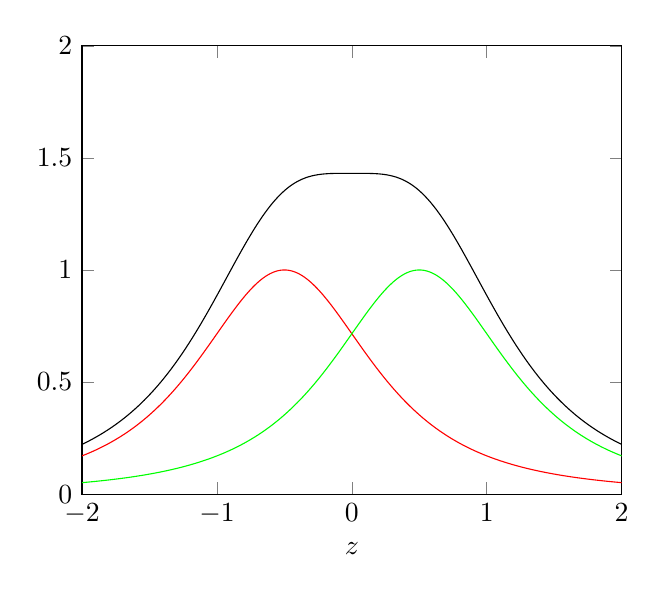
\begin{tikzpicture}
      \begin{axis}[
          domain=-2:2,
          xmin=-2, xmax=2,
          ymin=0, ymax=2,
          samples=400,
          xlabel=$z$
        ]
        \addplot[mark=none, red] {1/((x+1/2)^2+1)^(1.5)};
        \addplot[mark=none, green] {1/((x-1/2)^2+1)^(1.5)};
        \addplot[mark=none] {(1/((x-1/2)^2+1)^(1.5))+(1/((x+1/2)^2+1)^(1.5))};
      \end{axis}
    \end{tikzpicture}
    \caption{Helmholtz coil relative magnetic field strength. The coloured curves are the individual coils and the black curve is their sum.}
\end{figure}
and we see that indeed the field inside and near the center is highly uniform. Given that the uniformity is in such a small region I believe that 
a Taylor expansion or something similar on the $\bv{B}$ field could yield a simplified expression for the field in this region.
\end{soln}
\end{document}